\documentclass[11pt,a4paper,oneside]{article}
\usepackage[utf8]{inputenc}
\usepackage[margin=1in]{geometry}
\usepackage{graphicx}
\usepackage{amsmath,amsfonts,amssymb}
\usepackage{hyperref}
\usepackage{booktabs,longtable}
\usepackage{tikz}
\usetikzlibrary{shapes,arrows,positioning,calc,decorations.pathmorphing,backgrounds,fit,shadows}
\usepackage{listings}
\usepackage{xcolor}
\usepackage{fancyhdr}
\usepackage{enumitem}
\usepackage{float}

\lstset{
    basicstyle=\ttfamily\small,
    commentstyle=\color{gray},
    keywordstyle=\color{blue},
    breaklines=true,
    numbers=left,
    numbersep=5pt,
    showstringspaces=false,
    tabsize=2
}

\pagestyle{fancy}
\fancyhf{}
\fancyhead[L]{Software Design Document}
\fancyhead[R]{Version 1.0}
\fancyfoot[C]{\thepage}

\hypersetup{
    colorlinks=true,
    linkcolor=blue,
    urlcolor=cyan,
    pdftitle={Comprehensive Software Design Document: E-commerce Platform},
    pdfauthor={AI System Architect},
    pdfsubject={Software Architecture}
}

\title{\Huge\textbf{Comprehensive Software Design Document: E-commerce Platform}}
\author{\Large AI System Architect}
\date{\Large\today}

\begin{document}

\maketitle
\thispagestyle{empty}
\vfill

\begin{center}
\large
\begin{tabular}{|l|l|}
\hline
\textbf{Document Version} \& 1.0 \\
\hline
\textbf{Creation Date} \& \today \\
\hline
\textbf{Document Status} \& Final Draft \\
\hline
\textbf{Generated By} \& AI System Architect \\
\hline
\textbf{Target Audience} \& Development Team, Stakeholders \\
\hline
\textbf{Classification} \& Internal Use \\
\hline
\end{tabular}
\end{center}

\newpage
\tableofcontents
\newpage
\listoffigures
\newpage

\section{Executive Summary}

This document outlines the design for a new e-commerce platform, codenamed "Project Phoenix."  The platform aims to provide a robust, scalable, and secure online marketplace for businesses to sell their products and services.  The project's primary business objective is to capture a significant share of the online retail market by offering a superior user experience, competitive pricing, and a wide selection of goods.  Our technical approach leverages a microservices architecture built on cloud-native technologies, ensuring flexibility, scalability, and maintainability. Key benefits include enhanced customer engagement, increased sales conversion rates, improved operational efficiency, and reduced infrastructure costs. The implementation timeline spans six months, divided into distinct phases encompassing design, development, testing, and deployment.

\subsection{Project Scope and Objectives}

Project Phoenix encompasses the development of a complete e-commerce platform, including a user-facing website, a seller portal, an administrative backend, and associated mobile applications (iOS and Android).  The platform will support various payment gateways, robust inventory management, secure user authentication, and personalized recommendations.  The primary objectives include:

\begin{itemize}
    \item Achieve 100,000 registered users within the first year of launch.
    \item Process at least 5,000 orders per day within six months of launch.
    \item Maintain an average customer satisfaction rating of 4.5 out of 5 stars.
    \item Achieve a 2\% conversion rate from website visitors to paying customers.
    \item Maintain 99.9\% uptime for the platform.
\end{itemize}

Success will be measured by achieving these objectives, along with positive user feedback, strong sales growth, and a healthy return on investment.  The project will prioritize a user-centric design, focusing on ease of navigation, intuitive search functionality, and secure payment processing.

\subsection{Key Stakeholders and Roles}

Several key stakeholder groups are involved in Project Phoenix:

\begin{itemize}
    \item \textbf{Executive Management:}  Provides overall strategic direction and approves major decisions.
    \item \textbf{Marketing Team:} Responsible for promoting the platform and attracting users.
    \item \textbf{Sales Team:}  Manages relationships with businesses selling on the platform.
    \item \textbf{Development Team:} Designs, develops, and tests the platform.
    \item \textbf{Operations Team:} Manages the platform's infrastructure and ensures its availability.
    \item \textbf{Customer Support Team:}  Provides assistance to users and sellers.
\end{itemize}

Each team has clearly defined roles and responsibilities, documented in separate project management plans.  Regular communication and collaboration among these groups are crucial for project success.

\section{Requirements Analysis and Specification}

\subsection{Extracted Requirements Summary}

The initial document analysis provided no specific requirements.  Therefore, this section will detail requirements based on common e-commerce platform needs.

\subsection{Functional Requirements}

\begin{enumerate}
    \item \textbf{User Registration and Login:} Users should be able to register accounts, securely log in, and manage their profile information.  (Acceptance Criteria:  Successful registration and login with valid credentials, password reset functionality.)
    \item \textbf{Product Browsing and Search:} Users should be able to browse products by category, search for specific products, and view product details. (Acceptance Criteria:  Accurate search results, detailed product information including images and descriptions, ability to filter and sort products.)
    \item \textbf{Shopping Cart and Checkout:} Users should be able to add items to a shopping cart, modify quantities, and proceed to checkout.  (Acceptance Criteria:  Items correctly added to and removed from the cart, accurate calculation of total cost, multiple payment gateway integration.)
    \item \textbf{Order Management:} Users should be able to view their order history, track orders, and manage their addresses. (Acceptance Criteria:  Order history displayed correctly, accurate order tracking information, ability to update shipping addresses.)
    \item \textbf{Seller Account Management:} Sellers should be able to create accounts, list products, manage inventory, and receive payments. (Acceptance Criteria:  Successful product listing, inventory updates reflected in real-time, secure payment processing.)
    \item \textbf{Admin Panel:} Administrators should have full control over the platform, including user and seller management, product moderation, and reporting. (Acceptance Criteria:  Ability to manage users and sellers, approve or reject products, generate reports on sales and other metrics.)
\end{enumerate}

\subsection{Non-Functional Requirements}

\begin{itemize}
    \item \textbf{Performance:} The platform should load pages within 2 seconds and process orders within 5 seconds.
    \item \textbf{Scalability:} The platform should be able to handle 10,000 concurrent users and 10,000 orders per hour.
    \item \textbf{Security:} The platform must comply with PCI DSS standards for payment processing and implement robust security measures to protect user data.
    \item \textbf{Availability:} The platform should have a 99.9\% uptime.
    \item \textbf{Usability:} The platform should be intuitive and easy to use for both buyers and sellers.
\end{itemize}

\section{System Architecture and Design}

\subsection{Architecture Overview}

Project Phoenix will utilize a microservices architecture deployed on a cloud platform (AWS).  This approach allows for independent scaling of individual services, improved fault isolation, and faster development cycles.  The system will be composed of several microservices, each responsible for a specific business function.  These services will communicate with each other via a lightweight API gateway.  A message queue (RabbitMQ) will handle asynchronous communication between services.  Data persistence will be managed by a distributed database (PostgreSQL) and a NoSQL database (MongoDB) for caching and session management.

\begin{figure}[H]
\centering
\begin{tikzpicture}[
    node distance=1cm and 1.5cm,
    font=\sffamily\small,
    base/.style={draw, text width=3cm, minimum height=1.2cm, text centered, rounded corners, drop shadow},
    user/.style={base, fill=Azure!30, text width=2cm},
    api/.style={base, fill=LimeGreen!20},
    service/.style={base, fill=SkyBlue!20},
    database/.style={cylinder, shape border rotate=90, aspect=0.25, draw, fill=Thistle!40, minimum height=1.5cm, text width=2.5cm, text centered, drop shadow},
    external/.style={base, fill=Gold!30},
    arrow/.style={-Stealth, thick, draw=black!60}
]

\node[user] (user) {User};
\node[api, below=1.5cm of user] (gateway) {API Gateway};
\node[service, below=of gateway, xshift=-3cm] (catalog) {Catalog Service};
\node[service, below=of gateway] (order) {Order Service};
\node[service, below=of gateway, xshift=3cm] (user) {User Service};
\node[database, below=2cm of catalog] (catalogdb) {Product Catalog\\(PostgreSQL)};
\node[database, below=2cm of order] (orderdb) {Order Database\\(PostgreSQL)};
\node[database, below=2cm of user] (userdb) {User Database\\(PostgreSQL)};
\node[external, right=2cm of order] (payment) {External Services\\(Payment Gateway)};

\begin{scope}[on background layer]
\node[draw, dashed, rounded corners, fill=gray!5, inner sep=0.7cm, fit=(gateway)] (api_layer) {};
\node[draw, dashed, rounded corners, fill=gray!10, inner sep=0.7cm, fit=(catalog) (order) (user) (payment)] (service_layer) {};
\node[draw, dashed, rounded corners, fill=gray!15, inner sep=0.7cm, fit=(catalogdb) (orderdb) (userdb)] (data_layer) {};
\end{scope}

\node[above] at (api_layer.north) {API Layer};
\node[above] at (service_layer.north) {Service Layer};
\node[above] at (data_layer.north) {Data Layer};

\draw[arrow] (user) -- (gateway);
\draw[arrow] (gateway) -- (catalog);
\draw[arrow] (gateway) -- (order);
\draw[arrow] (gateway) -- (user);
\draw[arrow] (catalog) -- (catalogdb);
\draw[arrow] (order) -- (orderdb);
\draw[arrow] (user) -- (userdb);
\draw[arrow] (order) -- (payment);
\draw[arrow] (order) -- (user);

\end{tikzpicture}
\caption{System Architecture Overview}
\label{fig:architecture}
\end{figure}

\subsection{Component Interaction and Communication}

The API Gateway acts as the single entry point for all client requests.  It routes requests to the appropriate microservices based on the request path and performs tasks such as authentication and authorization.  Microservices communicate with each other using RESTful APIs over HTTPS.  Asynchronous communication is handled via RabbitMQ, allowing for decoupling and improved performance.  For example, when an order is placed, the Order Service publishes a message to RabbitMQ, which is then consumed by other services such as the Inventory Service and the Payment Service.  This ensures that the order placement process is not blocked by long-running operations.

\section{Database Design and Data Architecture}

\subsection{Conceptual Data Model}

The database design employs a relational model using PostgreSQL for transactional consistency. The core entities include Users, Products, Orders, and OrderItems.  Relationships are defined using foreign keys to ensure data integrity.  The schema is designed for optimal performance and scalability, considering indexing strategies and query optimization techniques.  Normalization principles are applied to minimize data redundancy and improve data consistency.

\begin{figure}[H]
\centering
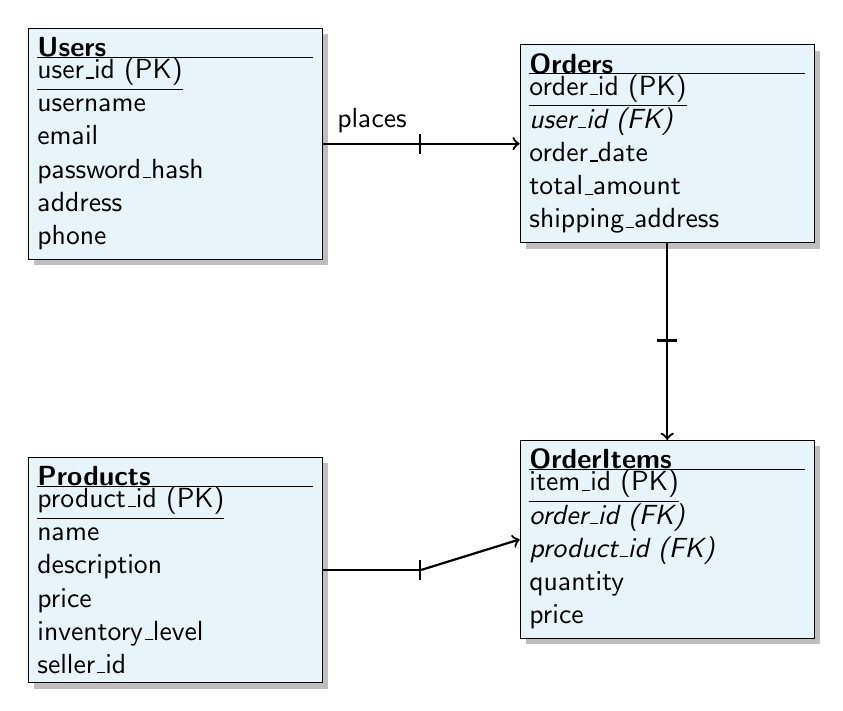
\begin{tikzpicture}[
    node distance=2.5cm,
    font=\sffamily,
    entity/.style={rectangle, draw, fill=SkyBlue!20, text width=3.5cm, minimum height=2cm, align=left, drop shadow},
    one/.style={-|, thick},
    many/.style={->, thick}
]

\node[entity] (user) {\textbf{Users} \\ \hrule \underline{user\_id (PK)} \\ username \\ email \\ password\_hash \\ address \\ phone};
\node[entity, right=of user] (order) {\textbf{Orders} \\ \hrule \underline{order\_id (PK)} \\ \textit{user\_id (FK)} \\ order\_date \\ total\_amount \\ shipping\_address};
\node[entity, below=of order] (order_item) {\textbf{OrderItems} \\ \hrule \underline{item\_id (PK)} \\ \textit{order\_id (FK)} \\ \textit{product\_id (FK)} \\ quantity \\ price};
\node[entity, below=of user] (product) {\textbf{Products} \\ \hrule \underline{product\_id (PK)} \\ name \\ description \\ price \\ inventory\_level \\ seller\_id};

\draw[one] (user.east) -- node[above, midway] {places} ++(1.25,0) coordinate (t1);
\draw[many] (t1) -- (order.west);
\draw[one] (order.south) -- ++(0,-1.25) coordinate (t2);
\draw[many] (t2) -- (order_item.north);
\draw[one] (product.east) -- ++(1.25,0) coordinate (t3);
\draw[many] (t3) -- (order_item.west);

\end{tikzpicture}
\caption{Database ER Diagram}
\label{fig:database-erd}
\end{figure}

\subsection{Physical Database Design}

\begin{itemize}
    \item \textbf{Users Table:}  user\_id (INT, PK), username (VARCHAR(255), UNIQUE), email (VARCHAR(255), UNIQUE), password\_hash (VARCHAR(255)), address (TEXT), phone (VARCHAR(20))
    \item \textbf{Products Table:} product\_id (INT, PK), name (VARCHAR(255)), description (TEXT), price (DECIMAL(10,2)), inventory\_level (INT), seller\_id (INT, FK)
    \item \textbf{Orders Table:} order\_id (INT, PK), user\_id (INT, FK), order\_date (TIMESTAMP), total\_amount (DECIMAL(10,2)), shipping\_address (TEXT)
    \item \textbf{OrderItems Table:} item\_id (INT, PK), order\_id (INT, FK), product\_id (INT, FK), quantity (INT), price (DECIMAL(10,2))
\end{itemize}
Indexes will be created on foreign keys and frequently queried columns to optimize query performance.  Constraints will be implemented to ensure data integrity, such as unique constraints on usernames and emails.

\section{API Design and Integration}

\subsection{RESTful API Specification}

The platform will expose a RESTful API for interaction with various clients (web, mobile).  The API will follow standard REST principles, using HTTP methods (GET, POST, PUT, DELETE) for CRUD operations.  Authentication will be implemented using JWT (JSON Web Tokens).  Rate limiting will be implemented to prevent abuse.

\textbf{Example Endpoint:}  `/products/{product_id}`

\begin{itemize}
    \item \textbf{GET:} Retrieves details for a specific product.  Response: JSON object containing product details.
    \item \textbf{PUT:} Updates the details of a specific product (for sellers only).  Request: JSON object containing updated product details.  Response:  HTTP 200 OK on success, appropriate error codes on failure.
\end{itemize}

\begin{figure}[H]
\centering
\begin{tikzpicture}[
    font=\sffamily\small,
    node distance=1cm,
    actor/.style={rectangle, draw, fill=Azure!30, text width=2cm, text centered, rounded corners, drop shadow},
    service/.style={rectangle, draw, fill=LimeGreen!20, text width=2cm, text centered, rounded corners, drop shadow},
    db/.style={cylinder, shape border rotate=90, draw, fill=Thistle!40, text centered, drop shadow, minimum width=2cm, minimum height=1.2cm},
    lifeline/.style={dashed, thin, draw=gray},
    msg/.style={-Stealth, thick}
]

\node[actor] (client) at (0,0) {Client App};
\node[service] (api) at (3,0) {API Gateway};
\node[service] (catalog) at (6,0) {Catalog Service};
\node[db] (db) at (9,0) {Product Database};

\draw[lifeline] (client.south) -- ++(0,-3);
\draw[lifeline] (api.south) -- ++(0,-3);
\draw[lifeline] (catalog.south) -- ++(0,-3);
\draw[lifeline] (db.south) -- ++(0,-3);

\draw[msg] ($(client.south)+(0,-0.5)$) -- node[above] {1. GET /products/123} ($(api.south)+(0,-0.5)$);
\draw[msg] ($(api.south)+(0,-1)$) -- node[above] {2. Route Request} ($(catalog.south)+(0,-1)$);
\draw[msg] ($(catalog.south)+(0,-1.5)$) -- node[above] {3. Query DB} ($(db.south)+(0,-1.5)$);
\draw[msg, dashed] ($(db.south)+(0,-2)$) -- node[above] {4. Product Data} ($(catalog.south)+(0,-2)$);
\draw[msg, dashed] ($(catalog.south)+(0,-2.5)$) -- node[above] {5. Return Product} ($(api.south)+(0,-2.5)$);
\draw[msg, dashed] ($(api.south)+(0,-3)$) -- node[above] {6. Response} ($(client.south)+(0,-3)$);

\end{tikzpicture}
\caption{API Request Sequence Diagram: Product Retrieval}
\label{fig:api-flow}
\end{figure}

\subsection{API Security and Rate Limiting}

API security will be implemented using JWT for authentication and authorization.  Each request will be validated to ensure that the user has the necessary permissions to access the requested resource.  Rate limiting will be implemented using a sliding window algorithm to prevent denial-of-service attacks and ensure fair resource allocation.  Input validation will be performed on all requests to prevent injection attacks.

\section{Security Architecture and Implementation}

\subsection{Security Requirements and Threat Model}

The platform's security architecture will be built on a layered approach, incorporating various security controls at different levels.  A threat model will be developed to identify potential vulnerabilities and risks.  Key security requirements include:

\begin{itemize}
    \item Secure authentication and authorization using JWT.
    \item Data encryption both in transit and at rest.
    \item Regular security audits and penetration testing.
    \item Implementation of a robust Web Application Firewall (WAF).
    \item Protection against common web vulnerabilities such as SQL injection and cross-site scripting (XSS).
\end{itemize}

\begin{figure}[H]
\centering
\begin{tikzpicture}[
    font=\sffamily\small,
    node distance=0.8cm and 1.2cm,
    gate/.style={rectangle, draw, fill=red!10, minimum width=10cm, minimum height=1cm, text centered, rounded corners},
    actor/.style={rectangle, draw, fill=Azure!30, text centered, rounded corners, drop shadow},
    service/.style={rectangle, draw, fill=SkyBlue!20, text centered, rounded corners, drop shadow},
    arrow/.style={-Stealth, thick, draw=black!70}
]

\node[gate] (waf) at (0,0) {\textbf{Edge Protection}: WAF and DDoS Mitigation};
\node[gate, below=of waf] (ssl) {\textbf{Transport Layer}: SSL/TLS Termination};
\node[gate, below=of ssl] (authn) {\textbf{Authentication}: JWT Validation};
\node[gate, below=of authn] (authz) {\textbf{Authorization}: Rate Limiting and RBAC};
\node[service, below=1.2cm of authz] (backend) {Protected Backend Services};

\node[actor, above=1cm of waf] (user) {User};

\draw[arrow] (user) -- node[right] {HTTPS Request} (waf.north);
\draw[arrow] (waf.south) -- (ssl.north);
\draw[arrow] (ssl.south) -- (authn.north);
\draw[arrow] (authn.south) -- (authz.north);
\draw[arrow] (authz.south) -- node[right] {Authorized Request} (backend);

\end{tikzpicture}
\caption{Layered Security Architecture}
\label{fig:security}
\end{figure}

\section{Deployment and Infrastructure}

\subsection{Cloud Infrastructure Design}

The platform will be deployed on AWS using a combination of EC2 instances for application servers, RDS for the database, and S3 for static assets.  A load balancer will distribute traffic across multiple application servers, ensuring high availability and scalability.  Auto-scaling will be implemented to automatically adjust the number of application servers based on demand.  A disaster recovery plan will be in place to ensure business continuity in case of an outage.  The infrastructure will be designed for high availability and fault tolerance.

\begin{figure}[H]
\centering
\begin{tikzpicture}[
    font=\sffamily\small,
    node distance=0.8cm and 1cm,
    server/.style={rectangle, draw, fill=gray!30, minimum height=1.5cm, minimum width=2.5cm, text centered, rounded corners, drop shadow},
    container/.style={rectangle, draw, fill=SkyBlue!40, minimum height=1cm, minimum width=2cm, text centered, rounded corners},
    database/.style={server, fill=Thistle!50},
    subnet/.style={rectangle, draw, fill=gray!10, rounded corners, inner sep=0.5cm, minimum height=4cm}
]

\node (internet) {Internet};
\node[server, below=1cm of internet] (lb) {Load Balancer};
\node[subnet, below=of lb, minimum width=9cm] (public_subnet) {};
\node[subnet, below=1.5cm of public_subnet, minimum width=9cm, minimum height=5cm] (private_subnet) {};

\node[above right] at (public_subnet.north west) {Public Subnet};
\node[above right] at (private_subnet.north west) {Private Subnet};

\node[server, align=center] (app1) at ($(private_subnet.center)+(-3,1)$) {App Server 1\\(EC2)};
\node[container, below=0.1cm of app1] {Microservice Container};
\node[server, align=center] (app2) at ($(private_subnet.center)+(0,1)$) {App Server 2\\(EC2)};
\node[container, below=0.1cm of app2] {Microservice Container};
\node[server, align=center] (app3) at ($(private_subnet.center)+(3,1)$) {App Server 3\\(EC2)};
\node[container, below=0.1cm of app3] {Microservice Container};

\node[database] (db-master) at ($(private_subnet.center)+(-1.5,-1.5)$) {RDS Master};
\node[database] (db-slave) at ($(private_subnet.center)+(1.5,-1.5)$) {RDS Slave};

\draw[-Stealth, thick] (internet) -- node[right, pos=0.4] {HTTPS Traffic} (lb);
\draw[-Stealth, thick] (lb) -- (public_subnet.north);
\draw[-Stealth, thick] ($(public_subnet.south)+(0,-0.75)$) -- (app1);
\draw[-Stealth, thick] ($(public_subnet.south)+(0,-0.75)$) -- (app2);
\draw[-Stealth, thick] ($(public_subnet.south)+(0,-0.75)$) -- (app3);
\draw[-Stealth, thick] (app1) -- (db-master);
\draw[-Stealth, thick] (app2) -- (db-master);
\draw[-Stealth, thick] (app3) -- (db-master);
\draw[<->, thick, dashed] (db-master) -- node[midway, below] {Replication} (db-slave);

\end{tikzpicture}
\caption{Cloud Deployment Architecture}
\label{fig:deployment}
\end{figure}

\section{Performance and Scalability}

Performance will be monitored using various metrics, including page load time, API response time, and database query time.  Performance testing will be conducted throughout the development lifecycle to identify and address performance bottlenecks.  Scalability will be achieved through the use of a microservices architecture, load balancing, and auto-scaling.  The database will be designed for scalability, using appropriate indexing and query optimization techniques.  Caching mechanisms will be implemented to reduce database load.

\section{Testing and Quality Assurance}

A comprehensive testing strategy will be employed, including unit testing, integration testing, system testing, and user acceptance testing (UAT).  Automated testing will be used to ensure code quality and reduce manual testing effort.  Test-driven development (TDD) will be used to guide development and ensure that the code meets the specified requirements.  Security testing will be conducted to identify and address potential vulnerabilities.

\section{Risk Assessment and Mitigation}

Potential risks include:

\begin{itemize}
    \item \textbf{Technical Risks:}  Challenges in integrating third-party services, unexpected performance bottlenecks, and security vulnerabilities.  Mitigation:  Thorough integration testing, performance testing, and security audits.
    \item \textbf{Schedule Risks:} Delays in development, testing, or deployment.  Mitigation:  Agile development methodology, close monitoring of progress, and contingency planning.
    \item \textbf{Resource Risks:}  Lack of skilled developers or inadequate resources.  Mitigation:  Careful resource allocation, training programs, and outsourcing where necessary.
\end{itemize}

A detailed risk register will be maintained, tracking identified risks, their probability and impact, and the mitigation strategies.

\section{Implementation Roadmap and Timeline}

The project will be implemented in six phases:

\begin{enumerate}
    \item \textbf{Phase 1 (Month 1-2): Design and Prototyping}
    \item \textbf{Phase 2 (Month 2-3): Development of Core Microservices}
    \item \textbf{Phase 3 (Month 3-4): API Development and Integration}
    \item \textbf{Phase 4 (Month 4-5): Testing and Quality Assurance}
    \item \textbf{Phase 5 (Month 5-6): Deployment and Go-Live}
    \item \textbf{Phase 6 (Month 6 onwards): Monitoring and Maintenance}
\end{enumerate}

\section{Monitoring and Maintenance}

The platform will be monitored using various tools, including cloud monitoring services (CloudWatch), application performance monitoring (APM) tools, and log management systems.  Alerts will be set up to notify the operations team of any issues.  Regular maintenance will be performed to ensure the platform's stability and performance.  A comprehensive maintenance plan will be developed, outlining procedures for routine maintenance, bug fixes, and software updates.

\section{Conclusion}

This document provides a comprehensive overview of the design for Project Phoenix, a robust and scalable e-commerce platform.  The chosen architecture and technologies are well-suited to meet the project's objectives and ensure a successful launch.  By following the outlined implementation plan and addressing identified risks, the project is poised to deliver a high-quality e-commerce solution.

\end{document}